In sensitivity analysis you vary one or more inputs systematically, drawing random numbers from distributions, such as the uniform or normal distribution. You run the simulation through many iterations and collect the outputs that you have chosen as response variables. Finally, you analyse to what degree the inputs determine the outputs, informally by visual methods or more formally by statistical methods, \eg\ through regression of the  outputs on the inputs.

\section{Setting up sensitivity analysis}
You prepare your box script for sensitivity analysis by including a \code{SensitivityAnalysisSimple} box at the top of the script and by defining statistical distributions for those inputs that you want to analyse (a more advanced \code{SensitivityAnalysisSobol} class has been implemented but remains to be documented). This is exemplified in the following script:

\lstset{numbers=left}
\begin{boxscript}
// sensitivity1.box
Simulation sim {
  .iterations = 5
  .steps = 35
  SensitivityAnalysisSimple {
    .method = "LHS"
  }
  Box butterfly {
    Stage egg {
      .initial = 100 
      .duration = 7 @(uniform 5 30)
      .k = 30 @(uniform 1 30)
    }
    Stage larva {
      .inflow = ../egg[outflow]
      .duration = 15
    }
    Stage pupa {
      .inflow = ../larva[outflow]
      .duration = 7
    }
    Stage adult {
      .inflow = ../pupa[outflow]
      .duration = 30
    }
  }
  OutputR {
    PageR {
      PlotR {
        .ports = (larva[content] pupa[content])
        .ggplot = "geom_point() + geom_line()"
      }
    }
  }
}
\end{boxscript}
\lstset{numbers=none}

Currently, two methods are available for sensitivity analysis: Latin Hypercube Sampling (LHS) and Monte Carlo (MC). LHS is the more effective one and is also the default setting. Here it has been set explicitly (line 6). The number of iterations in the sensitivity analysis is set in \code{Simulation} by the \code{iterations} port (line 3).

Two inputs have been chosen for the analysis (lines 11-12). You select a statistical distribution by the \code{@} operator. You can find the distributions available in \iref{ch:sensitivity-analysis-distributions}.  Here are some examples:
\lstset{numbers=left}
\begin{boxscript}
.i = 0 @ (uniform -7 8)
.j = 15.5 @ (normal 15 2)
.k = 14.9 @ (normal 15 2 0.05 0.9)
.l = 15.1 @ (normal 15 2 0 1)
\end{boxscript}
\lstset{numbers=none}
In line 1, \code{i} will be picked from the uniform distribution $[-7;8[$ (\ie\ closed downwards, open upwards). For example, \code{i} could have been declared as an integer (\code{int}) variable in the \CPP\ code. If you had a date as another input (\ie\ declared as a \code{QDate}), you could add \code{i} to that date and thereby obtain a random date inside a 14-days' interval (since \code{i} would take on values between $-7$ and 7, both numbers included).

In line 2, \code{j} will be picked from the normal distribution with a mean of 15 and standard deviation of 2. Line 3 specifies the same distribution albeit truncated, leaving only values between the 0.05 and 0.9 fractiles. The default fractiles are 0.01 and 0.99. So, in fact, line 2 specifies a truncated normal distribution as well. For a full normal distribution specify 0 and 1 fractiles as in line 4. The variables \code{j}, \code{k} and \code{l} would have been declared as \code{double} variables in the \CPP\ code.

Even though you specify a distribution with the \code{@} operator, you still need to set a default value as well (0, 15.5, 14.9 and 15.1 in lines 1-4). The \code{@} distributions take effect only if you have included a \code{SensitivityAnalysisSimple} box in the script. If there is no \code{SensitivityAnalysisSimple} box in the script then the default values are used instead of the \code{@} distributions. Thereby you can easily switch off all random \code{@} distributions, simply by removing (or commenting out) the \code{SensitivityAnalysisSimple} declaration (lines 5-7 in the script above).

\section{Uncertainty analysis}
The output (\iref{fig:sensitivity1}) that we got from the \filename{sensitivity1.box} script is not an illustration suitable for \concept{sensitivity analysis} but rather for \concept{uncertainty analysis}. In uncertainty analysis, variation in model outcome is studied in its own right without the aim to identify the most important sources of variation. 

In \iref{fig:sensitivity1} we have simply depicted the variation in simulation outcome given the variation in inputs without relating the outcome to the inputs. Note that the panels represent five iterations of the simulation, each simulation running for 35 steps. 

\begin{figure}
\centering
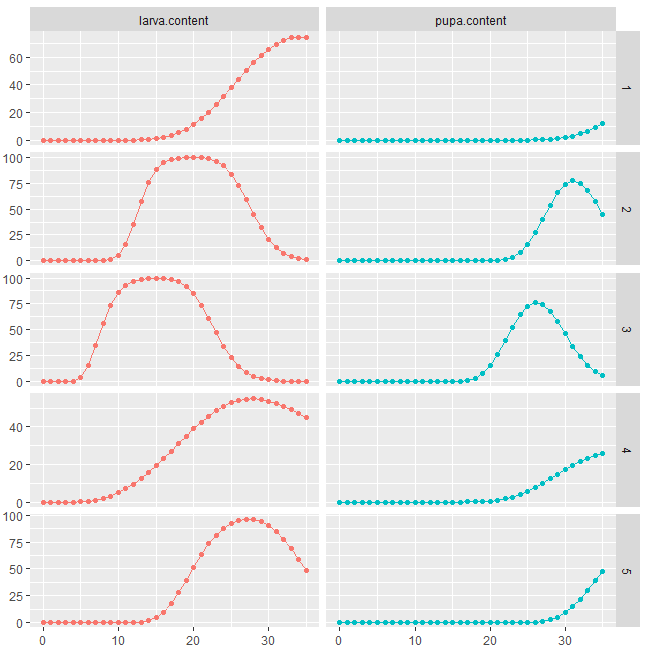
\includegraphics[scale=0.5]{graphics/sensitivity1}
\caption{Time trends produced by the \filename{\inputfolder/book/sensitivity1.box} script.}
\label{fig:sensitivity1}
\end{figure}

To continue the uncertainty analysis, we could make a phase plot of the two output variables studied (\code{larve[content]} and \code{pupa[content]}). For that purpose we only need to change the output settings:

\lstset{numbers=left}
\begin{boxscript}
// From sensitivity2.box
  OutputR {
    PageR {
      .xAxis = larva[content]
      PlotR {
        .layout = "merged" 
        .ports = pupa[content]
        .ggplot = "geom_point() + geom_path()"
      }             
    }
  }
}
\end{boxscript}
\lstset{numbers=none}

\begin{figure}
\centering
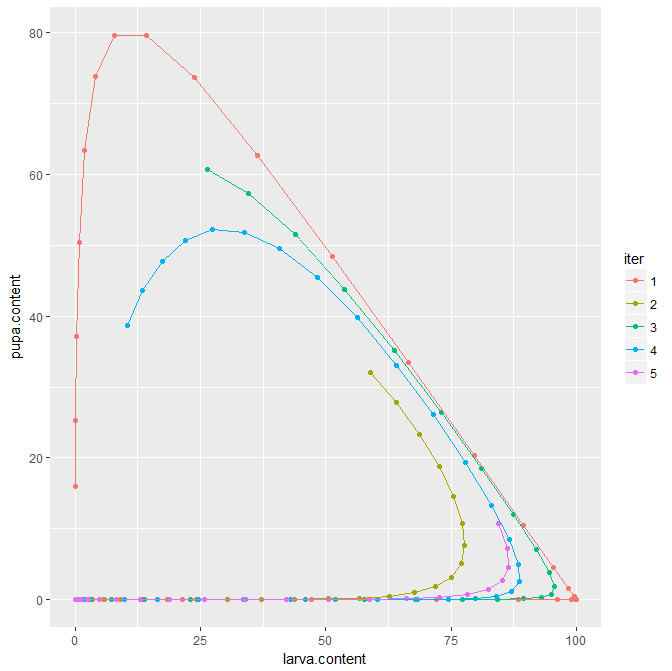
\includegraphics[scale=0.5]{graphics/sensitivity2}
\caption{Phase plot produced by the  \filename{\inputfolder/book/sensitivity2.box} script.}
\label{fig:sensitivity2}
\end{figure}

Here, we moved \code{larva[content]} from the $y$ to the \xaxis\ (line 4), thereby dropping time from either axis. However, the \code{geom_path()} (line 8) lets us follow time from point to point. We merge the iterations into one panel (line 6) to overlay and compare the iterations.

In the output (\iref{fig:sensitivity2}) we can see that not  only is the timing of the larva and pupa stages affected but so is their relative timing, since the phase plots do not overlap exactly. Each of the five curves is stringing 36 points together: one point for the initial values followed by 35 points for the following updates. 

The outputs shown in \iref{fig:sensitivity1} and \iref{fig:sensitivity2} do not match; they represent different random outcomes. If you want to produce matching figures, do it in one run. Put two \code{PageR} boxes, the one from \filename{sensitivity1.box} and the one from \filename{sensitivity2.box}, inside the \code{OutputR} box.

\section{Exploratory sensitivity analysis}
To carry out a sensitivity analysis proper, or at least to get started with the initial exploration of model sensitivities, we must put the randomised input variables on the \xaxis\ and the  output variables on the \yaxis. However, in our case the input variables have a fixed value throughout each iteration, whereas the output variables are vectors representing  time trends. 

To reduce the dimensions of this investigation, let's summarise the outputs by their final value in each iteration and put that value on the \yaxis. We can achieve this by changing only the output settings. To get some more output, now that we will only get one data point out of every iteration, let's also increase the number of iterations:

\lstset{numbers=left}
\begin{boxscript}
// From sensitivity3.box
Simulation sim {
  .iterations = 50
  :
  :
  OutputR {
    PageR {
      .xAxis = (egg[duration] egg[k])
      PlotR {
        .ports = (larva[content]|end pupa[content]|end)
        .ggplot = "geom_point() + geom_smooth()"
      }
    }
  }
}
\end{boxscript}
\lstset{numbers=none}

We have changed \code{iterations} to 50 (line 3) but what's more important; we have narrowed all outputs down to their final value (line 10). 

To turn port outputs (which are inherently vectors) into scalar values, we use the pipe operator (\code{|}) followed by the name of the operation we want to perform. There are five pipe operations to choose from:
\begin{compactitem}
\item{\codenobox{sum}}
\item{\codenobox{mean}}
\item{\codenobox{min}}
\item{\codenobox{max}}
\item{\codenobox{end}}
\end{compactitem}

\begin{figure} 
\centering
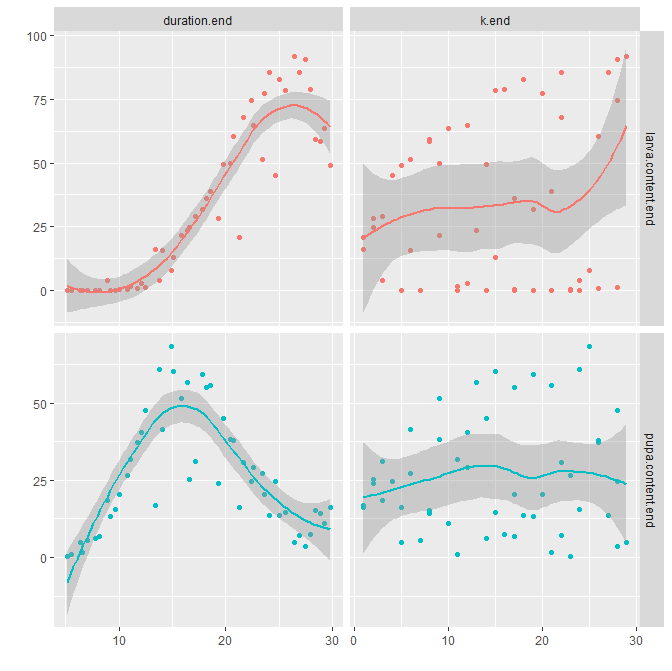
\includegraphics[scale=0.5]{graphics/sensitivity3}
\caption{Sensitivity analysis plots produced by the \filename{\inputfolder/book/sensitivity3.box} script.}
\label{fig:sensitivity3}
\end{figure}

Each operation summarises the vector as its name implies. In the script above we use \code{end} to obtain the last value of \code{larva[content]} and \code{pupa[content]} (line 10). For a final touch we apply \code{geom_smooth} (line 11) to obtain a trend curve through the plots.
                          
The outcome (\iref{fig:sensitivity3}) shows that the duration of the egg stage has a huge impact on the final number of larvae and pupae present (the two left-hand panels in the figure), while the $k$-value seems unimportant (the two right-hand panels of the figure), except maybe the variance of the output increases with increasing $k$.

Note that the \xaxis\ variables have also been led through the \code{end} pipe, as signified by their labels in the graph, \code{duration.end} and \code{k.end}. In general, if you pipe one output in a simulation, all of the other output ports must be piped too; otherwise there would be a mix of dimensions in the output. If some output ports have not been piped, they will default to the \code{end} pipe as seen here for the \xaxis\ ports. 

There exists a shorthand notation for putting all randomised variables on the \xaxis. You can replace line 8 above with the following one which uses a more generic specification of the \xaxis\ variables (see the \filename{\inputfolder/book/sensitivity4.box} script.):
\begin{boxscript}
.xAxis = *<Distribution>/..<Port>
\end{boxscript}

Here the \code{xAxis} (line 8 in the previous listing) is specified by a rather exotic path expression (see \iref{ch:path-expressions}). The first part (\code{*<Distribution>}) finds all objects of the class \code{Distribution}. Here, two such objects will be found, namely the two \code{uniform} objects. The second half of the path expression (\code{..<Port>}) finds the parent object for each of the \code{Distribution} objects just found. This parent must be of the \code{Port} class, as specified. You can use this \code{xAxis} specification as a starting point whenever you do sensitivity analysis. It will provide the output that you need for a first glance at the results.

\subsection{Available distributions}
\label{ch:sensitivity-analysis-distributions}
The statistical distributions available for sensitivity analysis are
\begin{itemize}
\item{\texttt{uniform}}
\item{\texttt{normal}}
\item{\texttt{loguniform}}
\item{\texttt{lognormal}}
\end{itemize}

You can find a demonstration of them in the \filename{\inputfolder/book/sensitivity5.box} script. Here is an excerpt:
\lstset{numbers=left}
\begin{boxscript}
Box inputs {
	+uniform = 0. @(uniform 0 30)
	+loguniform = 0. @(loguniform 0.001 1)
	+normal = 0. @(normal 100 10)
	+lognormal = 0. @(lognormal 100 0.5)
}
\end{boxscript}
\lstset{numbers=none}

The parameters for the two uniform distributions specify their minimum and maximum. For the two normal distributions, they specify first $\mu$ and then $\sigma$. Note that the \code{loguniform} distribution is uniform on a log-scale (here running from $-3$ to 0). Likewise, the \code{lognormal} distribution is normal on a log-scale. In \iref{fig:sensitivity5} you can see the shape of the generated distributions. 

For both log distributions, you provide their parameters on a linear scale, except for $\sigma$ of \code{lognormal}: The random numbers ($\overline{x}$) produced by \code{lognormal} will have an expected mean of $E\{mean(ln(\overline{x}))\}=ln(\mu)$ and an expected standard deviation of $E\{sd(ln(\overline{x}))\}=\sigma$.

\begin{figure} [t]
\centering
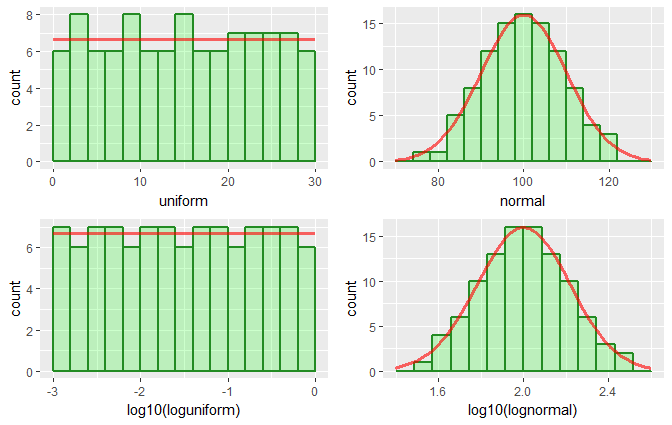
\includegraphics[width=.8\textwidth]{graphics/sensitivity5}
\caption{Statistical distributions available for sensitivity analysis. Produced by the \filename{\inputfolder/book/sensitivity5.box}  script.}
\label{fig:sensitivity5}
\end{figure}
